\documentclass[tikz,border=8pt]{standalone}
% Shared look for every TikZ diagram. Load with % Shared look for every TikZ diagram. Load with % Shared look for every TikZ diagram. Load with \input{../../tools/tikz-style.tex}
\usepackage[T1]{fontenc}
\usepackage{lmodern}
\renewcommand{\sfdefault}{lmr}  % diagrams use the same serif as the text
\usetikzlibrary{arrows.meta, positioning, shapes.geometric, calc, fit, backgrounds}
\definecolor{cblue}{HTML}{4C78A8}
\definecolor{corange}{HTML}{F58518}
\definecolor{cgreen}{HTML}{54A24B}
\definecolor{cred}{HTML}{E45756}
\definecolor{cpurple}{HTML}{B279A2}
\definecolor{cgrey}{HTML}{6B6B6B}
\tikzset{
  every picture/.style={font=\sffamily, line width=1.2pt},
  box/.style={draw=#1, fill=#1!12, rounded corners=4pt, align=center, inner sep=7pt, minimum height=1.1cm},
  box/.default=cgrey,
  arrow/.style={-{Stealth[length=3mm]}, draw=cgrey, line width=1.4pt},
  title/.style={font=\sffamily\bfseries\Large},
  note/.style={font=\sffamily\small, text=cgrey, align=center},
}
\AtBeginDocument{\hyphenpenalty=10000 \exhyphenpenalty=10000}

\usepackage[T1]{fontenc}
\usepackage{lmodern}
\renewcommand{\sfdefault}{lmr}  % diagrams use the same serif as the text
\usetikzlibrary{arrows.meta, positioning, shapes.geometric, calc, fit, backgrounds}
\definecolor{cblue}{HTML}{4C78A8}
\definecolor{corange}{HTML}{F58518}
\definecolor{cgreen}{HTML}{54A24B}
\definecolor{cred}{HTML}{E45756}
\definecolor{cpurple}{HTML}{B279A2}
\definecolor{cgrey}{HTML}{6B6B6B}
\tikzset{
  every picture/.style={font=\sffamily, line width=1.2pt},
  box/.style={draw=#1, fill=#1!12, rounded corners=4pt, align=center, inner sep=7pt, minimum height=1.1cm},
  box/.default=cgrey,
  arrow/.style={-{Stealth[length=3mm]}, draw=cgrey, line width=1.4pt},
  title/.style={font=\sffamily\bfseries\Large},
  note/.style={font=\sffamily\small, text=cgrey, align=center},
}
\AtBeginDocument{\hyphenpenalty=10000 \exhyphenpenalty=10000}

\usepackage[T1]{fontenc}
\usepackage{lmodern}
\renewcommand{\sfdefault}{lmr}  % diagrams use the same serif as the text
\usetikzlibrary{arrows.meta, positioning, shapes.geometric, calc, fit, backgrounds}
\definecolor{cblue}{HTML}{4C78A8}
\definecolor{corange}{HTML}{F58518}
\definecolor{cgreen}{HTML}{54A24B}
\definecolor{cred}{HTML}{E45756}
\definecolor{cpurple}{HTML}{B279A2}
\definecolor{cgrey}{HTML}{6B6B6B}
\tikzset{
  every picture/.style={font=\sffamily, line width=1.2pt},
  box/.style={draw=#1, fill=#1!12, rounded corners=4pt, align=center, inner sep=7pt, minimum height=1.1cm},
  box/.default=cgrey,
  arrow/.style={-{Stealth[length=3mm]}, draw=cgrey, line width=1.4pt},
  title/.style={font=\sffamily\bfseries\Large},
  note/.style={font=\sffamily\small, text=cgrey, align=center},
}
\AtBeginDocument{\hyphenpenalty=10000 \exhyphenpenalty=10000}

\begin{document}
\begin{tikzpicture}[
  q/.style={box=#1, minimum width=1.6cm, minimum height=1cm, font=\sffamily\large},
  link/.style={-{Stealth[length=3mm]}, draw=cred, line width=1.4pt},
  lab/.style={font=\sffamily\normalsize, text=cred, align=center}]
  \node[q=cred] (L) at (0,0) {$L$};
  \node[q=corange] (y) at (3.2,0) {$\hat{y}$};
  \node[q=corange] (zf) at (6.4,0) {$z_f$};
  \node[q=corange] (o) at (9.6,0) {$O_{11}$};
  \node[q=corange] (zp) at (12.8,0) {$z_p$};
  \node[q=cblue] (w) at (16.0,0) {$W^{1}_{11}$};
  \draw[link] (L) -- node[above=6pt, lab] {$\dfrac{\partial L}{\partial \hat y}$} (y);
  \draw[link] (y) -- node[above=6pt, lab] {$\dfrac{\partial \hat y}{\partial z_f}$} (zf);
  \draw[link] (zf) -- node[above=6pt, lab] {$\dfrac{\partial z_f}{\partial O_{11}}$} (o);
  \draw[link] (o) -- node[above=6pt, lab] {$\dfrac{\partial O_{11}}{\partial z_p}$} (zp);
  \draw[link] (zp) -- node[above=6pt, lab] {$\dfrac{\partial z_p}{\partial W^{1}_{11}}$} (w);
  % local derivatives
  \foreach \x/\t in {1.6/{$\dfrac{\hat y - y}{\hat y(1-\hat y)}$}, 4.8/{$\hat y(1-\hat y)$}, 8.0/{$W^{2}_{11}$},
                     11.2/{$O_{11}(1-O_{11})$}, 14.4/{$x_{i1}$}}
    \node[note, font=\sffamily\normalsize, text=black] at (\x,-1.3) {\t};
  \draw[decorate, decoration={brace, mirror, amplitude=6pt}, cgrey] (0.2,-2.1) -- (6.2,-2.1)
     node[midway, below=8pt, note, font=\sffamily\normalsize] {product: $-(y - \hat y)$};
  \node[note, font=\sffamily\normalsize] at (8,1.9) {gradient travels from the loss back to the weight; each arrow multiplies by its local derivative};
\end{tikzpicture}
\end{document}
